% Это основная команда, с которой начинается любой \LaTeX-файл. Она отвечает за тип документа, с которым связаны основные правил оформления текста.
\documentclass{article}

% Здесь идет преамбула документа, тут пишутся команды, которые настраивают LaTeX окружение, подключаете внешние пакеты, определяете свои команды и окружения. В данном случае я это делаю в отдельных файлах, а тут подключаю эти файлы.

% Здесь я подключаю разные стилевые пакеты. Например возможности набирать особые символы или возможность компилировать русский текст. Подробное описание внутри.
\usepackage{packages}

% Здесь я определяю разные окружения, например, теоремы, определения, замечания и так далее. У этих окружений разные стили оформления, кроме того, эти окружения могут быть нумерованными или нет. Все подробно объяснено внутри.
\usepackage{environments}

% Мое
\usepackage{mathtools}
\usepackage{tikz}
\makeatletter
\newcommand\mathcircled[1]{%
  \mathpalette\@mathcircled{#1}%
}

\newcommand\@mathcircled[2]{%
  \tikz[baseline=(math.base)] \node[draw,circle,inner sep=1pt] (math) {$\m@th#1#2$};%
}
\makeatother

\usepackage{mathrsfs}

\usepackage{listings}
% \usepackage{xcolor}

\definecolor{backcolour}{rgb}{0.95,0.95,0.92}
\definecolor{codegreen}{rgb}{0,0.6,0}

\lstdefinestyle{myStyle}{
    backgroundcolor=\color{backcolour},
    commentstyle=\color{codegreen},
    basicstyle=\ttfamily\footnotesize,
    breakatwhitespace=false,
    breaklines=true,
    keepspaces=true,
    numbers=left,
    numbersep=5pt,
    showspaces=false,
    showstringspaces=false,
    showtabs=false,
    tabsize=2,
}

\lstset{style=myStyle}


% Здесь я определяю разные команды, которых нет в LaTeX, но мне нужны, например, команда \tr для обозначения следа матрицы. Или я переопределяю LaTeX команды, которые работают не так, как мне хотелось бы. Типичный пример мнимая и вещественная часть комплексного числа \Im, \Re. В оригинале они выглядят не так, как мы привыкли. Кроме того, \Im еще используется и для обозначения образа линейного отображения. Подробнее описано внутри.
\usepackage{commands}

% Пакет для титульника проекта
\usepackage{titlepage}

% Здесь задаем параметры титульной страницы
\setUDK{192.168.1.1}
% Выбрать одно из двух
% \setToResearch
\setToProgram

\setTitle{Нейросети с нуля}

% Выбрать одно из трех:
% КТ1 -- \setStageOne
% КТ2 -- \setStageTwo
% Финальная версия -- \setStageFinal
% \setStageOne
%\setStageTwo
\setStageFinal

\setGroup{204}
%сюда можно воткнуть картинку подписи
\setStudentSgn{
\includegraphics[scale=0.15]{pictures/sgn.jpeg}}
\setStudent{Артур Маратович Гимранов}
\setStudentDate{19.05.2022}
\setAdvisor{Дмитрий Витальевич Трушин}
\setAdvisorTitle{доцент, к.ф.-м.н.}
\setAdvisorAffiliation{ФКН НИУ ВШЭ}
\setAdvisorDate{22 мая}
\setGrade{9}
%сюда можно воткнуть картинку подписи
\setAdvisorSgn{\smash{
\includegraphics[scale=0.17]{pictures/trushin_sgn.png}}}
\setYear{2022}


% С этого момента начинается текст документа
\begin{document}

% Эта команда создает титульную страницу
\makeTitlePage

% Здесь будет автоматически генерироваться содержание документа
\tableofcontents

% Данное окружение оформляет аннотацию: краткое описание текста выделенным абзацем после заголовка

\newpage

\begin{abstract}
В рамках этого проекта предполагается изучить теорию нейросетей и их обучения и написать проект в котором будут реализованы все необходимые компоненты для работы и обучения нейросети.
\end{abstract}


\section{Введение}
\begin{center}
    \href{https://github.com/toobrainless/NeuralNetwork}{Репозиторий на github}.
\end{center}

Нейронная сеть -- это набор нейронов и связей между ними. Структура нейронной сети пришла в программирование прямиком из биологии, где она встречается в виде устройства нервной системы живых существ.

В качестве примера можно рассмотреть зрачковый рефлекс. В нашем глазу есть сенсоры, которые улавливают количество света попадающего через зрачок. Отсюда импульс на сужение зрачка пойдет к нервным окончаниям. Таким образом, нейронная сеть, получив сигнал от фоторецепторов, обрабатывает данную информацию и принимает решение какие мышцы задействовать для ответной реакции, то есть сузить или расширить зрачок.

Нейрон лучшего всего представлять как функцию с множеством входов и одним выходом. Его задача взять числа с входов, преобразовать их каким-то образом и передать дальше.

Между нейронами есть связи -- это каналы которые имеют вес и передают выход одного нейрона на вход другому с определенным весом.

\begin{figure}[h]
\center{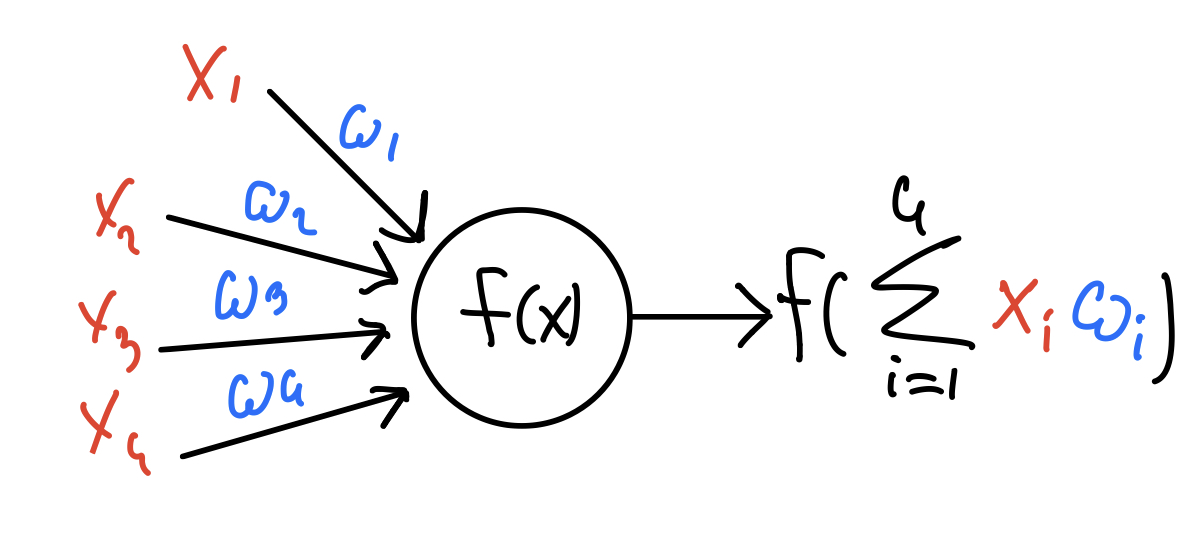
\includegraphics[scale=0.15]{pictures/neuron.jpeg}}
\caption{Устройство нейрона}
\end{figure}

Чтобы придать дополнительную структуру, нейроны укладывают в слои, где внутри одного слоя нейроны не связаны, но связаны со следующим и предыдущим.

\begin{figure}[h]
    \center{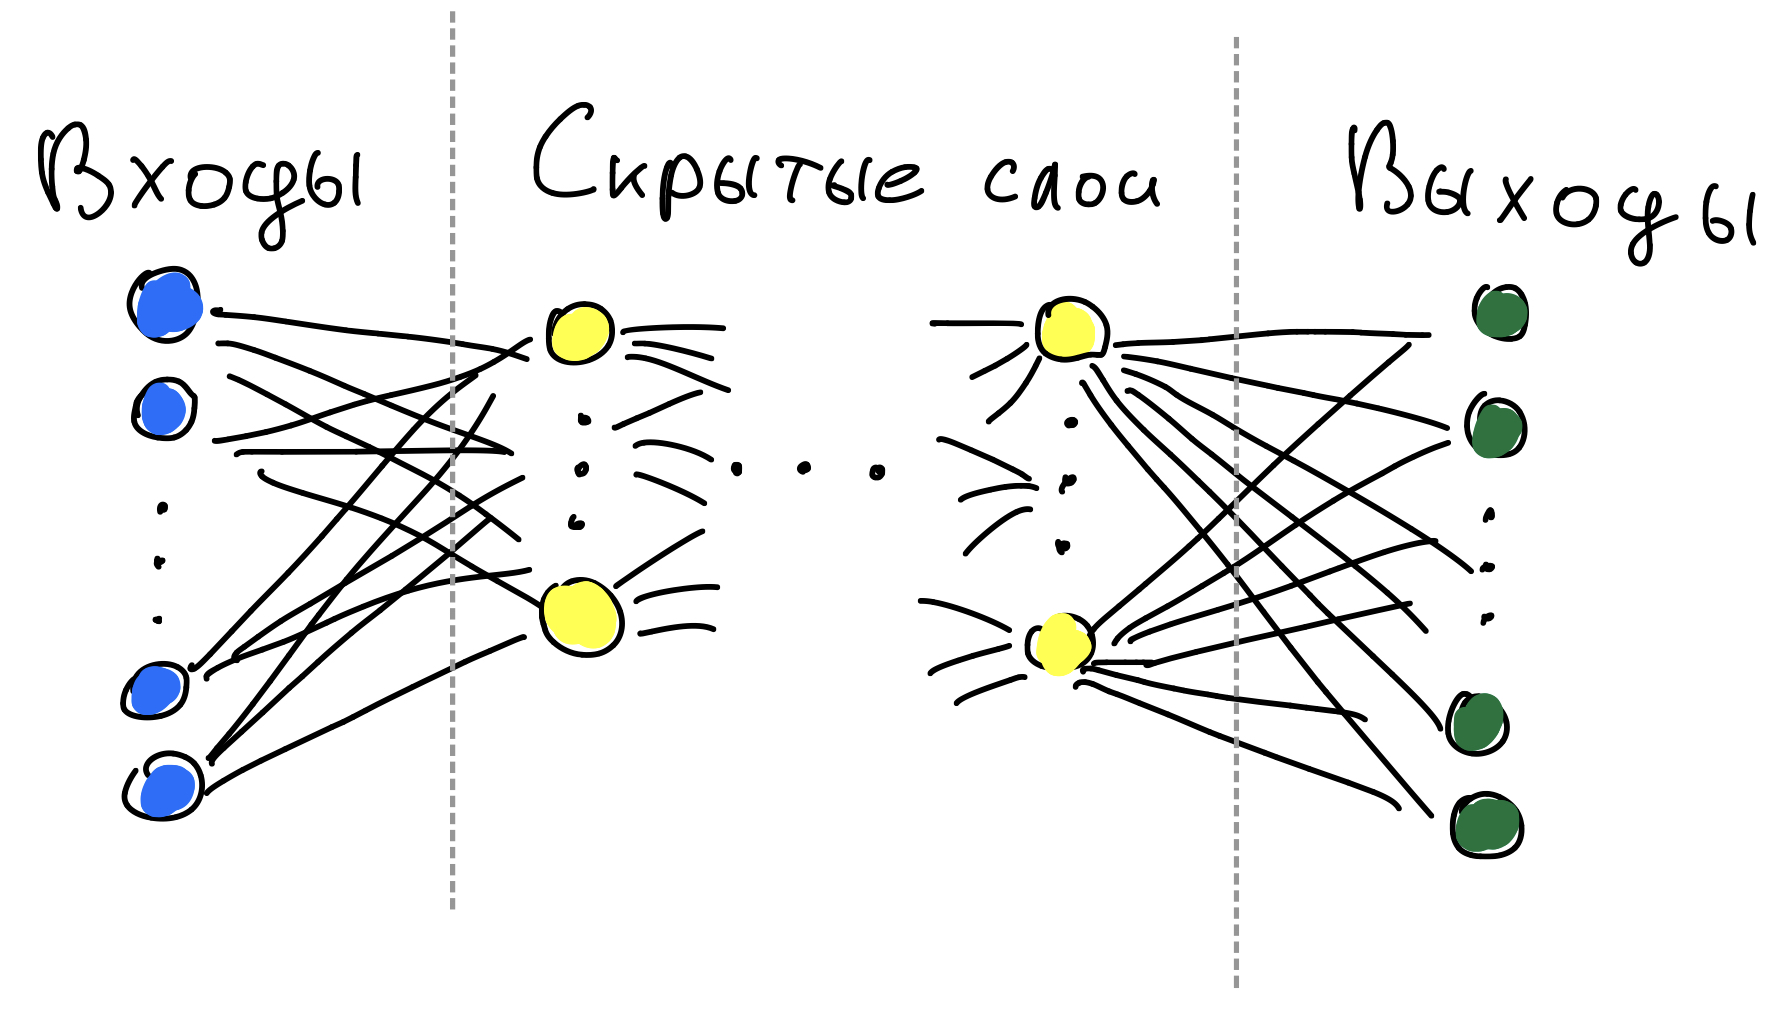
\includegraphics[scale=0.15]{pictures/structure.jpeg}}
    \caption{Структура нейросети}
\end{figure}

Таким образом наша сеть представляет собой направленный ациклический граф. Где данные идут в одном направлении -- от входов к выходам. Это сеть прямого распространения, а если быть точным многослойный перцептрон.

% Реализовывать это все будем с помощью матричного умножения. Представим наш слой в виде блока, который хранит параметры нашей функции и саму функцию

% $$
% \rightarrow \underset{f(x, \theta_1)}{\boxed{\theta_1}} \rightarrow
% $$

% Параметры это веса связей и смещение,
Теперь надо обучить сеть на специальной, размеченной выборке. Назначим все веса случайным образом и посмотрим что нам выдаст наша сетка. Зная результат работы нейросети и правильные ответы для наших входов пройдемся в обратном порядке по всем нейронам и поменяем параметры, чтобы уменьшить ошибку, часть нейронов будем учитывать с меньшим весом, а другую часть с большим. Через какое-то количество таких итераций, наша сетка научится выдавать правильные предсказания по обучающей выборке, потом только стоит протестировать ее на другой выборке и оценить точность.

Перенесем это все на язык математики и программирования. Посмотрим на взаимодействия двух соседних слоев. Пусть в текущем слое $m$ нейронов его выходы будут $y_i$, а в предыдущем $n$ нейронов, выходы $x_i$. Тогда можем посчитать $y_i = f\left(\Sum{j = 1}{n}w_{ij}x_j + b_i \right)$, где $w_{ij}$ связь между $j$-ым нейроном предыдущего слоя и $i$-ым нейроном текущего слоя, $b_i$ -- сдвиг, добавим его для большей гибкости, а $f$ -- функция активации нейрона. Можем переписать это все на матричном языке, как $y = f(Ax + b)$, $A$ -- содержит веса, $b$ -- сдвиги, а $f$ мы применяем поэлементно. Представим наш слой в виде блока, который хранит параметры $\theta = (A, b)$ и $f$.
$$
\R^n \xrightarrow[]{x} \underset{f(x, \theta)}{\boxed{\theta}} \xrightarrow[]{y} \R^m
$$
Теперь о задаче, которую мы решаем. Пусть у нас есть $k$ признаков, которые уложены в вектор $x = [x^{(1)}, \dots, x^{(k)}]^t$, по которым мы хотим предсказать результат $y$ у которого тоже есть свои $l$ признаков $y = [y^{(1)}, \dots, y^{(l)}]^t$, аналогично запишем их в вектор. Тогда хотим выразить $y$ через $x$ в виде функции $F(x) = y$. Понятно, что для $n$ векторов и образов эта задача решается очень легко, нам же хочется обучить модель по начальной выборке, чтобы ошибка на векторах не из обучающей выборке была минимальна. Вот тут и вступает в дело наша нейросеть, именно в таком виде будем искать эту функцию $F$.

Для примера рассмотрим сетку из двух слоев. Пусть у нас есть два блока с параметрами $\theta_1, \theta_2$ и у нас выполняется такая цепочка функций

$$
\R^n \xrightarrow[]{x_i} \underset{f(x, \theta_1)}{\boxed{\theta_1}} \xrightarrow[]{w_i} \underset{g(x, \theta_2)}{\boxed{\theta_2}} \xrightarrow[]{z_i} \R^m
$$
Тогда мы хотим подобрать такие параметры $\theta_1, \theta_2$, чтобы минимизировать ошибку на обучающей выборке $x_i \in \R^n, y_i \in \R^m$.
$$
\begin{bmatrix}
x_1\\
\vdots\\
x_p
\end{bmatrix}
\rightarrow
\begin{bmatrix}
y_1\\
\vdots\\
y_p
\end{bmatrix}
$$
Добавим функцию ошибки $\phi(\theta_1, \theta_2) = \Sum{i = 1}{p} \|g(f(x_i, \theta_1), \theta_2) - y_i\|^2 \rightarrow \underline{\min}$, чтобы понимать что мы хотим уменьшать. Теперь мы хотим посчитать градиент по параметрам $\theta_1, \theta_2$ и градиентным спуском минимизирвать ошибку.

Таким образом, в проекте я реализую следующие компоненты: узел нейросети, который состоит из линейного отображения и нелинейной части, объекты отвечающие функциям штрафа. Будет реализован механизм вычисления градиента для узла и проталкивания градиента в узлы предыдущего слоя. На основе этого механизма будут написаны методы обучения нейросети. Передо мной стоят следующие задачи:
\begin{enumerate}
    \item изучить теорию нейросетей и градиентоного спуска
    \item кратко изложить в отчете теорию
    \item имплементировать необходимые классы и структуры
    \item изложить в отчете архитектуру и дизайн имплементации
    \item написать сопроводительную документацию.
\end{enumerate}

\section{Важный пример}

Рассмотрим задачу. Допустим мы хотим найти зависимость цены квартиры от некоторого набора параметров: жилой площади, расстояния до метро, расстояния до центра. Представьте, что мы измерили все эти параметры для $n$ квартир и получили наборы значений. Цену сложим в $y_i$, а параметры в вектора
$x_i =[x_i^{(1)}, x_i^{(2)}, x_i^{(3)}]^t$. И мы хотим подобрать функцию $f$, чтобы $f(x_i) = y_i$. Конечно нет строгой зависимости подходящей любой квартире, но мы можем подобрать функцию в некотором виде, для которой отклонение в наших точках было бы наименьшим:

$$
\Sum{i = 0}{n} |f(x_i) - y_i| \rightarrow \min
$$

% \section{Описание функциональных и нефункциональных требований к программному проекту}
\section{Функциональные требования}
Наша программа будет получать на вход обучающую выборку подбирать по ней параметры и вычислять предполагаемое значение в точке.
\begin{enumerate}
\item \texttt{Net}. Инцилизирует ресурсы, слои нейронки и блок функции ошибок. Главный класс проекта, нужен для обучения и предсказания значения в точке.
\item \texttt{ComputeBlock}.  Те самые слои нейронки или наши "блоки". Содержит функцию и ее параметры. Умеет вычислять функцию в точке, считать градиент по параметрам и проталкивать его в следующий блок.
\item \texttt{LosFunction}. Функция ошибок, нужна для расчета отклонения и вычисления градиента
\item \texttt{ActivationFunction}. Класс родитель для функций активации, имеет виртуальные методы для вычисления функции и ее производной в точке. Ниже перечислены ее наследники, в них должны быть имплементированы фукнции для вычисления и взятия производной.
    \begin{enumerate}
        \item \texttt{Sigmoid}
        \item \texttt{Relu}
        \item \texttt{Softmax}
    \end{enumerate}
\end{enumerate}

\section{Нефункциональные требования}

\begin{itemize}
    \item C++20~\cite{cpp}
    \item Google C++ Style Guide~\cite{styleguide}
    \item ClangFormat linter~\cite{clangformat}
    \item Библиотека Eigen~\cite{eigen} для работы с матрицами
    \item Система поддержки версий: git~\cite{git} с github~\cite{github}
\end{itemize}

% \section{Основная часть}

\section{Нейросети}

\subsection{Теория}
Сеть
$$
\R^n \rightarrow \underset{f_1(x, \theta_1)}{\boxed
{\theta_1}} \rightarrow \dots \rightarrow \underset{f_i(x, \theta_i)}{\boxed{\theta_i}} \rightarrow \dots \rightarrow \underset{f_k(x, \theta_k)}{\boxed
{\theta_k}} \rightarrow \mathcircled{\mathscr{L}} \rightarrow \R
$$
Где $f_i(x) = \phi(A_ix + b_i)$, $\phi(x)$ -- функция активации, $(A_i, b_i) = \theta_i$ -- параметры блока, $\mathscr{L}$ -- функция потерь. Пусть $F_{\Theta}(x)$, $\Theta = (\theta_1, \dots, \theta_k)$ функция предсказания, то есть $F_{\Theta}$ передает выход $i$ блока на вход $i + 1$, пока не дойдет до последнего блока и не посчитает предсказываемый результат. Более формально, будем рекуррентно строить функции $F_{\Theta, i}(x) = f_i(F_{\Theta, i - 1}(x), \theta_i)$, $F_{\Theta, 1}(x) = f_1(x, \theta_1)$, обозначим $F_\Theta(x) = F_{\Theta, n}(x)$. Тогда функция которую мы хотим минимизировать $\psi(\Theta) = \frac{1}{n} \Sum{i = 1}{n} \mathscr{L}(F_{\Theta}(x_i), y_i)$.

Цель заключается в том, чтобы пройти вперед, посчитать предсказание, отдать его в функцию потерь, и посчитать градиент по параметрам обратным проходом.

Нам надо уметь считать $\frac{\partial \psi}{\partial \theta_j}$.

$$
\frac{\partial \psi}{\partial \theta_j} = \frac{1}{n}\Sum{i = 1}{n} \left(\frac{\partial \mathscr{L}(F_{\Theta}(x_i), y_i)}{\partial F_{\Theta}(x_i)} \frac{\partial F_{\Theta}(x_i)}{\partial \theta_j}\right)
$$

\begin{center}
$\frac{\partial \mathscr{L}(z, y)}{\partial z}$ -- считается в зависимости от функции потерь.
\end{center}
$$
\frac{\partial F_{\Theta}(x)}{\partial \theta_i} = \Prod{j = 0}{n - i + 1} \left( \frac{\partial f_{n - j}(F_{\Theta, n - j - 1}(x)), \theta_{n - j})}{\partial F_{\Theta, n - j - 1}(x)} \right) \cdot \frac{\partial f_i(F_{\Theta, i - 1}(x), \theta_i)}{\partial \theta_i}
$$

Последнее выражение мы будем считать поэтапно, идя в обратную сторону по нашим блокам, сначала посчитаем для последнего, там это просто превращается в $\frac{\partial F_{\Theta, n}}{\partial \theta_n} = \frac{\partial f_n(F_{\Theta, n - 1}(x), \theta_n)}{\partial \theta_n}$, дальше будет нарастать произведение $\Prod{j = 0}{n - i + 1} \left( \frac{\partial f_{n - j}(F_{\Theta, n - j - 1}(x)), \theta_{n - j})}{\partial F_{\Theta, n - j - 1}(x)} \right)$, множители которого мы будем передавать в следущий блок из текущего. Например для перехода от последнего блока к предпоследнему, $\frac{\partial F_{\Theta, n}}{\partial \theta_{n - 1}} = \frac{f_n(F_{\Theta, n - 1}(x), \theta_n)}{\partial F_{\Theta, n - 1}(x)} \cdot \frac{\partial f_{n - 1}(F_{\Theta, n - 2}(x), \theta_{n - 1})}{\partial \theta_{n - 1}}$, тут первое слагаемое пришло из последнего блока, а второе слагаемое относится к предпоследнему блоку. Продемонстрирую на картинке, для наглядности.
% \newpage
\begin{figure}[h]
    \center{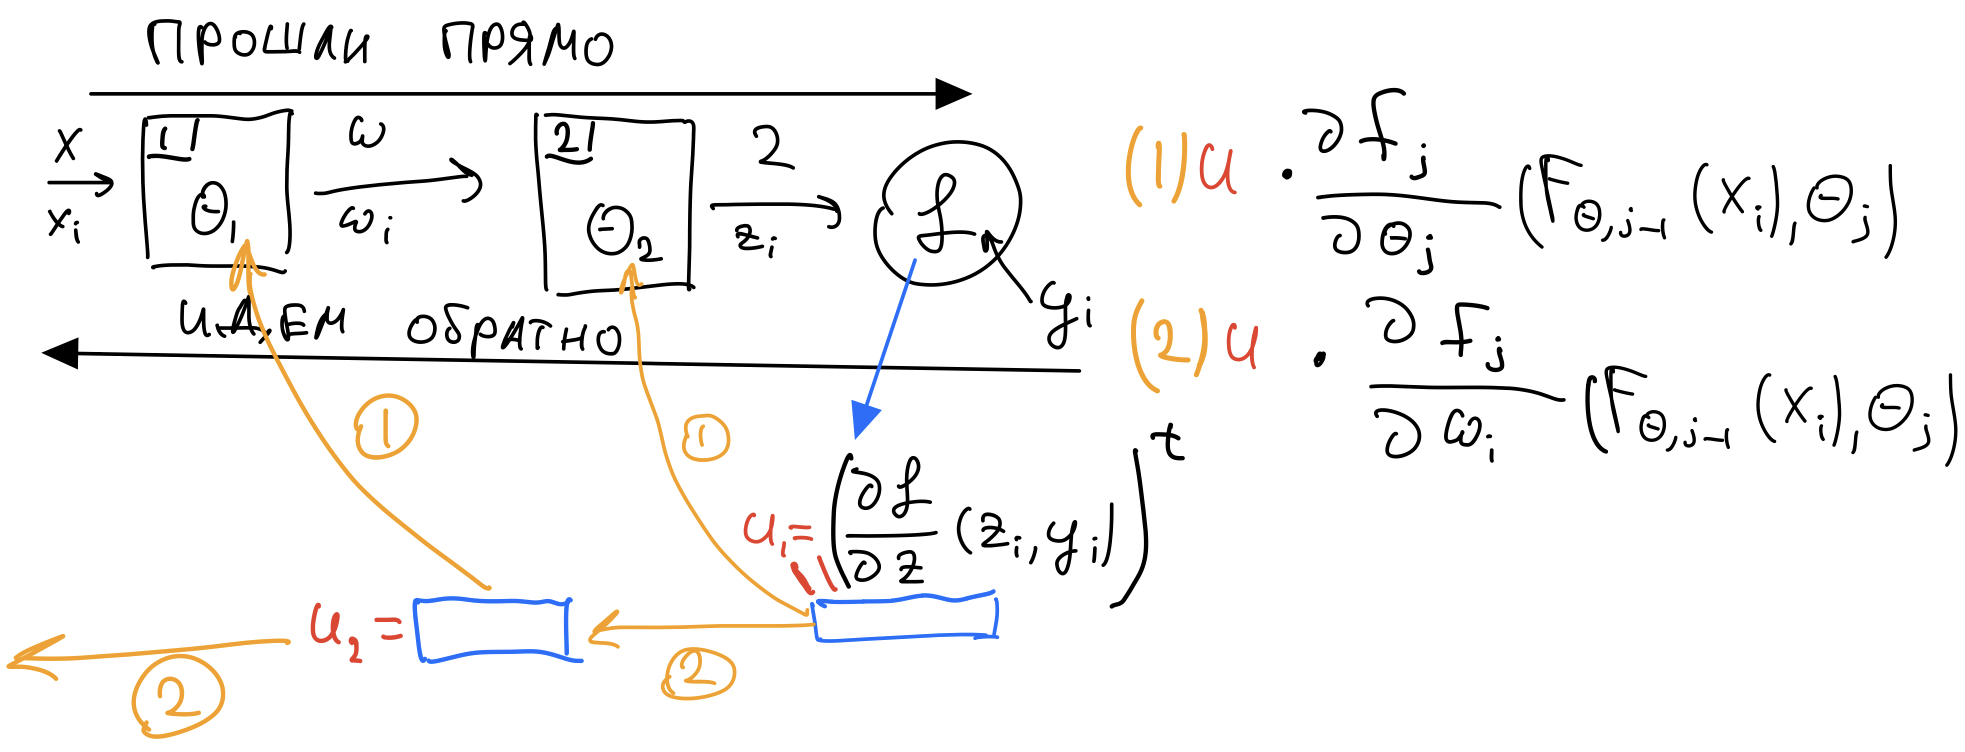
\includegraphics[scale=0.25]{pictures/grad_expl.jpg}}
    \caption{Структура нейросети}
\end{figure}

Тут мы сразу считаем градиент по параметрам с учетом функции потерь. Считаем $u_1 = \left(\frac{\partial \mathscr{L}(z_i, y_i)}{\partial z}\right)^t$ и прокидываем дальше. Теперь считаем градиент по $\theta_2$ как $u_1 \cdot \frac{\partial f_2(w_i, \theta_2)}{\partial \theta_2}$ и $u_2 = u_1 \cdot \frac{\partial f_2(w_i, \theta_2)}{\partial w_i}$, прокидываем $u_2$ дальше и аналогично считаем градиенты по параметрам следующих блоков.

Осталось научиться считать градиенты

$$
u^t\frac{\partial f(x, \theta)}{\partial x}, u^t\frac{\partial f(x, \theta)}{\partial \theta} = \left(u^t\frac{\partial f(x, \theta)}{\partial A}, u^t\frac{\partial f(x, \theta)}{\partial b} \right)
$$

$$
f(x, A, b) = \phi(A_ix + b_i)
$$

$$
u^td(\phi(Ax + b)) = u^t\phi'(Ax + b)d(Ax + b) = u^t\phi'(Ax + b)db = \langle\left(u^t\phi'(Ax + b)\right)^t, db\rangle \Rightarrow u^t\frac{\partial f(x, \theta)}{\partial b} = \phi'(Ax + b)^tu
$$
$$
u^td(\phi(Ax + b)) = u^t\phi'(Ax + b)d(Ax + b) = u^t\phi'(Ax + b)(dA)x = \tr\left(u^t\phi'(Ax + b)(dA)x\right) = \tr\left(xu^t\phi'(Ax + b)(dA)\right) \mathcircled{=}
$$
$$
\mathcircled{=} \langle\left(xu^t\phi'(Ax + b)\right)^t , dA\rangle_F \Rightarrow u^t\frac{\partial f(x, \theta)}{\partial A} = \phi'(Ax + b)^tux^t
$$
$$
u^td(\phi(Ax + b)) = u^t\phi'(Ax + b)d(Ax + b) = u^t\phi'Adx = \langle(u^t\phi'(Ax + b)A)^t, dx\rangle \Rightarrow u^t\frac{\partial f(x, \theta)}{\partial x} = A^t\phi'(Ax + b)u
$$

За функцию потерь я взял MSE, то есть $\mathscr{L}(z, y) = \|z - y\|_2^2 = (z - y)^t(z - y)$

$$
d\mathscr{L}(z, y) = 2(z - y)^tdx, \frac{\partial \mathscr{L}(z, y)}{\partial z} = 2(z - y)
$$

И рассмотрел три функции активации.\\

\textbf{sigmoid}
$$
\sigma(x) = \frac{1}{1 + e^{-x}}
$$
$$
\sigma'(x) = \frac{e^{-x}}{(e^{-x} + 1)^2}
$$

К вектору мы применяем ее поэлементно, тогда $\frac{\partial \sigma(x)}{\partial x}, x \in \R^n$ будет диагональная матрица, у которой на диагонали стоят $\sigma'(x_i)$, а все остальное по нулям

\textbf{relu}

Так как я столкнулся с проблемой "умирающего релу", было принято решение не занулять $x$ в отрицательной части

$$
\relu(x)
=
\begin{cases}
    x, & x > 0 \\
    0.01x, & x \le 0
\end{cases}
$$

$$
\relu'(x)
=
\begin{cases}
    1, & x > 0 \\
    0.01, & x \le 0
\end{cases}
$$

Аналогично sigmoid'e, $\frac{\partial \relu(x)}{\partial x}, x \in \R^n$ будет диагональная матрциа, у которой на диагонали стоят $\relu'(x_i)$, а все остальное по нулям

\textbf{softmax}

$$
\softmax(x)_i = \frac{e^{x_i}}{\Sum{j = 1}{n}e^{x_j}}, x \in \R^n
$$

Для

$$
\frac{\partial \softmax(x)}{\partial x} =
\begin{bmatrix}{}
    \frac{\partial s_{1}}{\partial x_{1}} & \frac{\partial s_{1}}{\partial x_{2}} & \cdots & \frac{\partial s_{1}}{\partial x_{n}} \\
    \frac{\partial s_{2}}{\partial x_{1}} & \frac{\partial s_{2}}{\partial x_{2}} & \cdots & \frac{\partial s_{2}}{\partial x_{n}} \\
    \vdots & \vdots & \ddots & \vdots \\
    \frac{\partial s_{n}}{\partial x_{1}} & \frac{\partial s_{n}}{\partial x_{2}} & \cdots & \frac{\partial s_{n}}{\partial x_{n}}
\end{bmatrix},
s_i = \softmax(x)_i
$$

Теперь, так как производная это аддитивная функция, мы можем отдельно посчитать $\frac{\partial \mathscr{L}(F_\Theta(x_i), y_i)}{\partial \theta_j}$, для каждого $x_i$, усреднить и получить $\frac{\partial \psi}{\partial \theta_i}$ и теперь с правильно подобранным шагом градиентного спуска (learning rate), идти против градиента, тем самым уменьшая нашу ошибку
$$
\theta_i' = \theta_i - lr \cdot \frac{\partial \psi}{\partial \theta_i}
$$

\subsection{Net}
Главный класс сети. Содержит в себе слои и функцию потерь. Распределяет все данные между слоями. Выполняет обучение сети с последующим предсказанием результата. Пройдемся по ключевым функциям.

\begin{itemize}
    \item В конструкторе мы задаем размеры слоев, функцию активации для каждого слоя, количество итераций обучения, размер батча для стохастического градиентного спуска и шаг градиентного спуска
    \item \texttt{train} -- начинает процесс обучения по выборке. На вход принимает две матрицы $x$ -- по столбикам содержит параметры, $y$ -- по столбикам содержит выходы, для данных параметров
    \item \texttt{predict\_1d} -- по параметрам выдает предсказание
    \item \texttt{predict\_2d} -- принимает на вход матрицу у которой по столбцам вектора параметров, возвращает матрицу в которой по столбцам лежат соотвествующие предсказания
    \item \texttt{push\_forward} -- делает прямой проход, считает все выходы и итоговое предсказание
    \item \texttt{back\_propagate} -- запускает обратное распространение, считает нужные градиенты по параметрам и входам, проталкивает их дальше
    \item \texttt{update\_parameters} -- обновляет параметры после обратного распространения, принимает на вход шаг градиентного спуска
\end{itemize}


\subsection{ComputeBlock}
Слой нейронной сети. Содержат параметры $\theta = (A, b)$ и функцию активации $\phi$. Нужен для вычисления функции $f(x) = \phi(Ax + b)$, и градиентов $\frac{\partial f}{\partial A}, \frac{\partial f}{\partial b}, \frac{\partial f}{\partial x}$. Также обновляет параметры по заданному шагу спуска и размеру батча
\begin{itemize}
    \item В конструкторе получает функцию активации, размеры матрицы и инцилизирует $A$ и $b$ случайными числами из равномерного распределения на $[-1, 1]$
    \item \texttt{evaluate\_1d} -- по переданному вектору вычисляет функцию $f(x) = \phi(Ax + b)$ и возвращает результат
    \item \texttt{evaluate\_2d} -- аналогично версии \texttt{1d}, только принимает матрицу и возвращает матрицу, в которой по столбцам лежат результаты
    \item \texttt{push\_forward} -- продолжает прямой подход в текущем блоке
    \item \texttt{back\_propagate} -- продолжает обратное распространение в текущем блоке
    \item \texttt{update\_parameters} -- обновляет свои параметру после обратного распространения
    \item \texttt{grad\_A} -- вычисляет $\frac{\partial f}{\partial A}$
    \item \texttt{grad\_b} -- вычисляет $\frac{\partial f}{\partial b}$
    \item \texttt{grad\_x} -- вычисляет $\frac{\partial f}{\partial x}$
\end{itemize}

\subsection{Функции активации}

Реализованы $\softmax, \relu, \sigmoid$ у всех трех функций имплементированы функии \texttt{evaluate} и \texttt{derivative}, для вычисления функции и производной в точке

\subsection{Функция потерь}
В качестве функции потерь была взята MSE

\begin{itemize}
    \item \texttt{evaluate\_1d} -- вычисляет функцию ошибки по двум векторам $z, y$
    \item \texttt{evaluate\_2d} -- вычисляет функцию ошибки по двум матрицам $z, y$ как среднее функций ошибок для соответствующих столбцов
    \item \texttt{grad\_z} -- вычисляет $\frac{\partial \mathscr{L}(z, y)}{\partial z}$
\end{itemize}

\section{Итоги}

Была изучена теория нейронных сетей и градиентного спуска, полностью реализован функционал нейросети.
\subsection*{Тест}
Проект был протестирован на датасете mnist ~\cite{mnist}, и показал на нем точность более 90\%.
\subsubsection*{Входные данные}
\begin{itemize}
    \item Сеть обучалась на выборке из 8500 размеченных изображениях рукописных цифр
    \item Входной слой состоял из 784 нейронов, каждый из которых отвечал за пиксель в картинке $28 \times 28$, с функцией активации $\relu$
    \item Первый скрытый слой состоял из 16 нейронов, с функцией активации $\relu$
    \item Второй скрытый слой состоял из 16 нейронов, с функцией активации $\softmax$
    \item Выходной слой состоял из 10 нейронов
    \item Количество эпох (итераций обучения) = 3000
    \item Learning rate (шаг градиентного спуска) = 0.6
    \item Размер батча 128
    \item Функция потерь MSE
\end{itemize}

Из начальной выборки на каждой итерации обучения случайным образом выбиралось 128 векторов на которых мы считали ошибку и обучали. В первых двух слоях были выбраны функции активации $\relu$, так как градиент $\sigmoid$ы быстро затухал и сеть переставала обучаться. Второй скрытый слой был с функцией активации $\softmax$, она хорошо подходит для принятия решения "голосованием". на выходе был вектор из 10 координат и нейроны "голосовали"\ за координаты, индекс координаты с наибольшим весом и являлся ответом. Процесс обучения на CPU занял 12 минут.

После обучения выборка была протестирована на 1500 других изображений рукописных цифр, и правильно определила цифру на 1351 изображении, таким образом точность составила чуть больше 90\%.



% Здесь идет планомерное изложение информации от начала до конца. Тут не нужна никакая философия или объяснения, все это было во введении. Тут сухой математический текст с определениями, формулировками и где надо доказательствами. Содержательную часть можно бить на части, чтобы структурировать изложение.

% \subsection{Содержательная часть 1}

% \subsection{Содержательная часть 2}

% Здесь автоматически генерируется библиография. Первая команда задает стиль оформления библиографии, а вторая указывает на имя файла с расширением bib, в котором находится информация об источниках.
\bibliographystyle{plainurl}
\bibliography{bibl}



% % С этого момента глобальная нумерация идет буквами. Этот раздел я добавил лишь для демонстрации возможностей LaTeX, его можно и нужно удалить и он не нужен для курсового проекта непосредственно.
% \appendix

% Проведем небольшой обзор возможностей \LaTeX. Далее идет обзорный кусок, который надо будет вырезать. Он приведен лишь для демонстрации возможностей \LaTeX.

% \section{Нумеруемый заголовок}
% Текст раздела
% \subsection{Нумеруемый подзаголовок}
% Текст подраздела
% \subsubsection{Нумеруемый подподзаголовок}
% Текст подподраздела

% \section*{Не нумеруемый заголовок}
% Текст раздела
% \subsection*{Не нумеруемый подзаголовок}
% Текст подраздела
% \subsubsection*{Не нумеруемый подподзаголовок}
% Текст подподраздела


% \paragraph{Заголовок абзаца} Текст абзаца

% Формулы в тексте набирают так $x = e^{\pi i}\sqrt{\text{формула}}$. Выключенные не нумерованные формулы набираются либо так:
% \[
% x = e^{\pi i}\sqrt{\text{формула}}
% \]
% Либо так
% $$
% x = e^{\pi i}\sqrt{\text{формула}}
% $$
% Первый способ предпочтительнее при подаче статей в журналы AMS, потому рекомендую привыкать к нему.

% Выключенные нумерованные формулы:
% \begin{equation}\label{Equation1}
% % \label{имя-метки} эта команда ставит метку, на которую потом можно сослаться с помощью \ref{имя-метки}. Метки можно ставить на все объекты, у которых есть автоматические счетчики (номера разделов, подразделов, теорем, лемм, формул и т.д.
% x = e^{\pi i}\sqrt{\text{формула}}
% \end{equation}
% Или не нумерованная версия
% \begin{equation*}
% x = e^{\pi i}\sqrt{\text{формула}}
% \end{equation*}

% Уравнение~\ref{Equation1} радостно занумеровано.

% Лесенка для длинных формул
% \begin{multline}
% x = e^{\pi i}\sqrt{\text{очень очень очень длинная формула}}=\\
% \tr A - \sin(\text{еще одна очень очень длинная формула})=\\
% \cos z \Im \varphi(\text{и последняя длинная при длинная формула})
% \end{multline}

% Многострочная формула с центровкой
% \begin{gather}
% x = e^{\pi i}\sqrt{\text{очень очень очень длинная формула}}=\\
% \tr A - \sin(\text{еще одна очень очень длинная формула})=\\
% \cos z \Im \varphi(\text{и последняя длинная при длинная формула})
% \end{gather}

% Многострочная формула с ручным выравниванием. Выравнивание идет по знаку $\&$, который на печать не выводится.
% \begin{align}
% x = &e^{\pi i}\sqrt{\text{очень очень очень длинная формула}}=\\
% &\tr A - \sin(\text{еще одна очень очень длинная формула})=\\
% &\cos z \Im \varphi(\text{и последняя длинная при длинная формула})
% \end{align}

% \begin{theorem}
% Текст теоремы
% \end{theorem}
% \begin{proof}
% В специальном окружении оформляется доказательство.
% \end{proof}

% \begin{theorem}[Имя теоремы]
% Текст теоремы
% \end{theorem}
% \begin{proof}[Доказательство нашей теоремы]
% В специальном окружении оформляется доказательство.
% \end{proof}

% \begin{definition}
% Текст определения
% \end{definition}

% \begin{remark}
% Текст замечания
% \end{remark}

% \paragraph{Перечни:} Нумерованные
% \begin{enumerate}
% \item Первый
% \item Второй
% \begin{enumerate}
% \item Вложенный первый
% \item Вложенный второй
% \end{enumerate}
% \end{enumerate}

% Не нумерованные

% \begin{itemize}
% \item Первый
% \item Второй
% \begin{itemize}
% \item Вложенный первый
% \item Вложенный второй
% \end{itemize}
% \end{itemize}


% Здесь текст документа заканчивается
\end{document}
% Начиная с этого момента весь текст LaTeX игнорирует, можете вставлять любую абракадабру.
